\section{Work Plan - placeholder}
\subsection{Mark Allocation}

iv. \textbf{Work Plan -- 10\%}

\textit{show the processes, milestones and dependencies}

\subsection{Detail Task Description} 

vi. plan the steps required to complete the work and the dependencies between them in detail through a \textit{graphical work plan};

\subsection{Proposal Structure}

A work-plan showing the steps required to complete the work. This must be presented in graphical form.

Markers will look for the extent to which: tasks are identified comprehensively and in detail; timings are realistic; dependencies are considered and milestones set; the work-plan is comprehensive, coherent and aligned with the rest of the proposal; the work plan is legible*, comprehensive, realistic, aligned with project objectives and suggests that the project is likely to succeed;

*We receive a surprising number of work-plans that are highly pixelated screen dumps of tiny unreadable text. Marks will not be awarded for illegible plans.

\subsection{Processes, milestones and dependencies.}

\textbf{Dependencies} are the relationships among tasks which determine the order in which activities need to be performed. There are four (4) types of dependency relationships. From  

https://www.projectinsight.net/project-management-basics/task-dependencies

A project \textbf{milestone} is a task of zero duration that shows an important achievement in a project. The milestones should represent a clear sequence of events that incrementally build up until your project is complete.

https://www.clarizen.com/what-are-project-milestones/

The workplan, see Figure \ref{fig:example}. 

\begin{figure}[ht]
\centering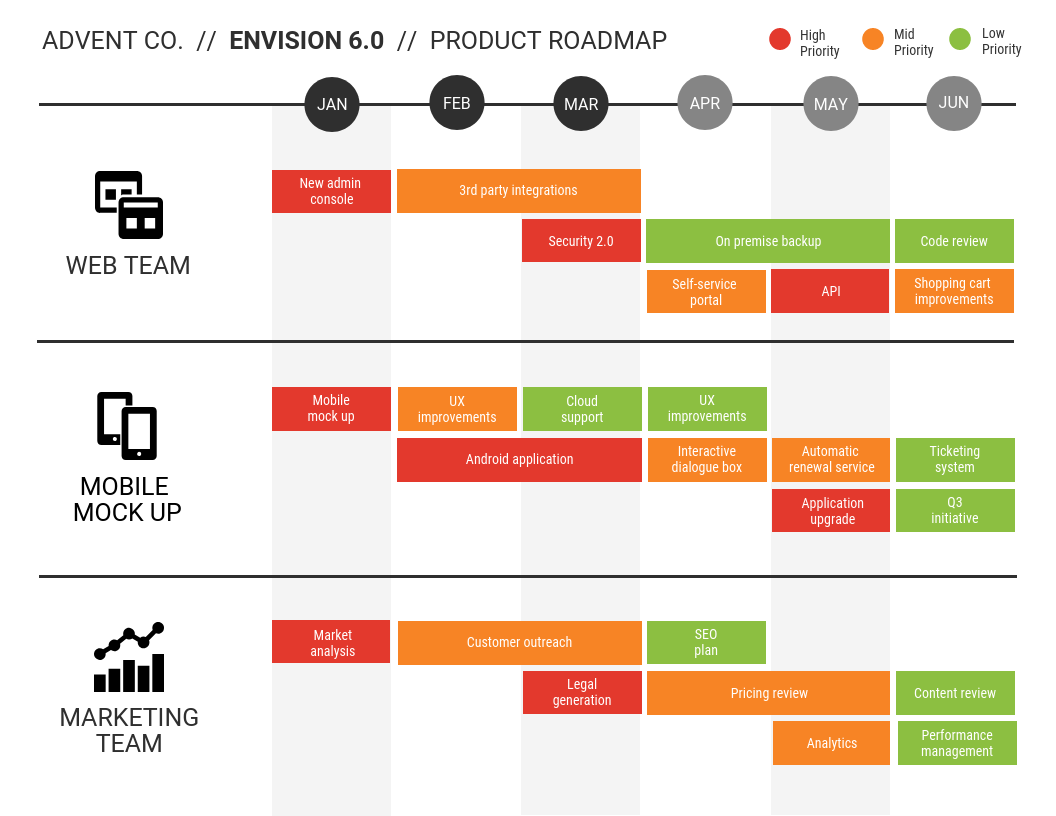
\includegraphics[width=1\linewidth]{project-plan-template-10.png}
\caption{Graphical Work Plan - Project Title - image needs to be much smaller}
\label{fig:workplan}
\end{figure}